\part{The Blinn-Phong illumination model}
\frame{\partpage}

\begin{frame}{The Blinn-Phong illumination model}
	\pause Jim Blinn,
	``Models of light reflection for computer synthesized pictures''.
	\textit{ACM SIGGRAPH Computer Graphics},
	11(2):192--198,
	1977.
	
	\begin{itemize}
		\pause\item The Blinn-Phong model builds on the Phong shading model
		\pause\item It breaks lighting down into three parts: \textbf{ambient}, \textbf{diffuse}, and \textbf{specular}.
	\end{itemize}
	\pause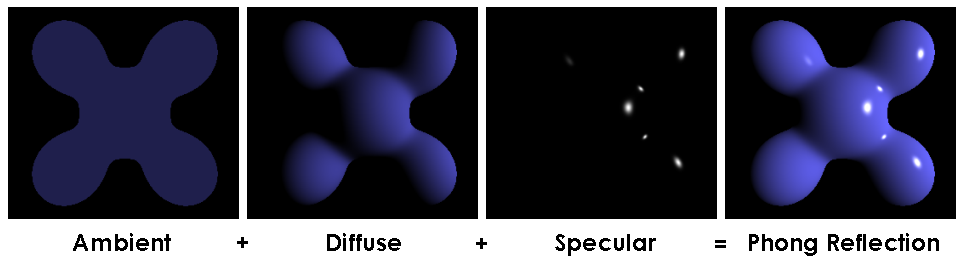
\includegraphics[width=\textwidth]{phong}
\end{frame}

\begin{frame}{Diffuse lighting}
	\pause
	\begin{columns}
		\begin{column}{0.33\textwidth}
			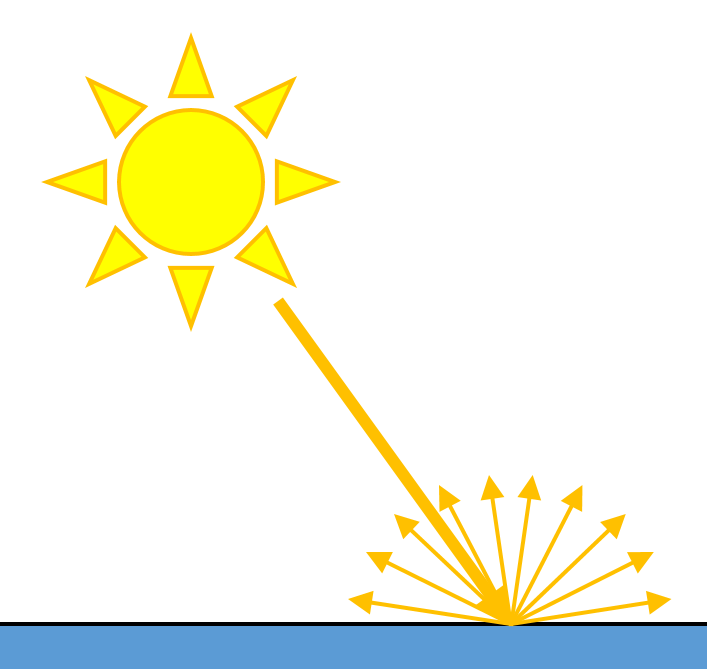
\includegraphics[width=\textwidth]{diffuse_1}
		\end{column}
		\begin{column}{0.65\textwidth}
			When light hits a ``rough'' surface, it is \textbf{scattered equally in all directions}
		\end{column}
	\end{columns}
	\pause
	\begin{columns}
		\begin{column}{0.65\textwidth}
			The amount of light hitting the surface depends on the \textbf{angle} between the surface and the light source
		\end{column}
		\begin{column}{0.33\textwidth}
			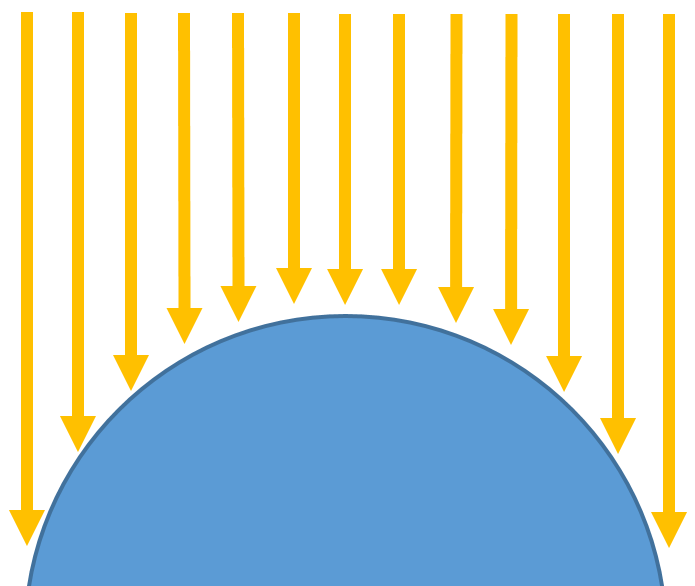
\includegraphics[width=\textwidth]{diffuse_2}
		\end{column}
	\end{columns}
\end{frame}

\begin{frame}{Diffuse lighting formula}
	\begin{columns}
		\begin{column}{0.25\textwidth}
			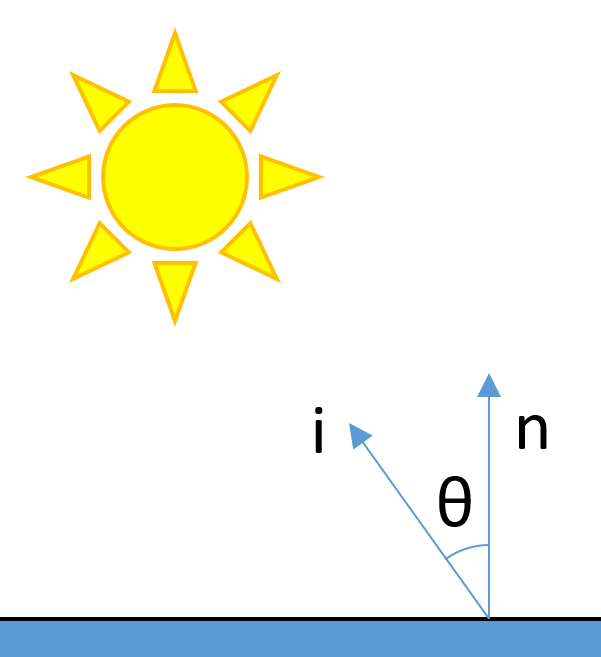
\includegraphics[width=\textwidth]{diffuse_angle}
		\end{column}
		\begin{column}{0.73\textwidth}
			\begin{itemize}
				\pause\item Light intensity is proportional to the \textbf{cosine} of the angle between the \textbf{light direction} and the \textbf{surface normal}
				\pause\item Let $n$ be the normal, and $i$ be a unit vector pointing towards the light source
				\pause\item Light intensity is proportional to
					$\cos \theta = n \cdot i$
				\pause\item If the surface is \textbf{pointing away} from the light source, we get $\theta > \frac{\pi}{2}$ so $\cos \theta < 0$ ---
					in this case we \textbf{clamp} the answer to $0$
			\end{itemize}
		\end{column}
	\end{columns}
\end{frame}

\begin{frame}{Light direction and intensity}
	\begin{itemize}
		\pause\item For a distant light source (e.g.\ the sun), direction and intensity are \textbf{constant}
		\begin{itemize}
			\pause\item These are known as \textbf{directional} lights
		\end{itemize}
		\pause\item For a \textbf{point} light source (e.g.\ a lightbulb):
			\begin{itemize}
				\pause\item Direction is calculated by subtracting the fragment position from the light position
				\pause\item Intensity is usually \textbf{attenuated}, e.g. using an \textbf{inverse square law}: if the distance between the fragment and the light source is $d$, then the light intensity is proportional to $\frac{1}{d^2}$
			\end{itemize}
	\end{itemize}
\end{frame}

\begin{frame}{Specular lighting}
	\pause
	\begin{columns}
		\begin{column}{0.33\textwidth}
			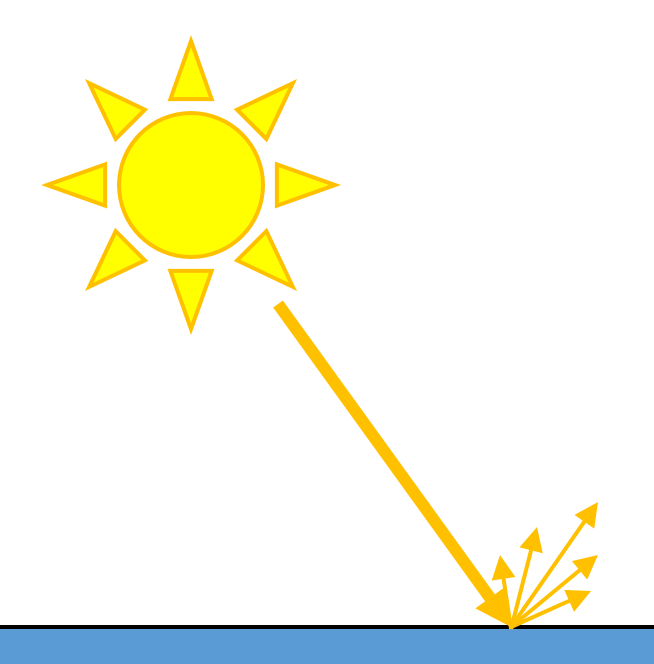
\includegraphics[width=\textwidth]{specular_1}
		\end{column}
		\begin{column}{0.65\textwidth}
			\begin{itemize}
				\pause\item When light hits a ``smooth'' surface, it is \textbf{reflected} across a narrow range of angles
				\pause\item This creates a \textbf{specular highlight}, with intensity dependent on the \textbf{view direction} as well as the direction to the light source.
			\end{itemize}
		\end{column}
	\end{columns}
\end{frame}

\begin{frame}{Specular lighting formula}
	\begin{columns}
		\begin{column}{0.33\textwidth}
			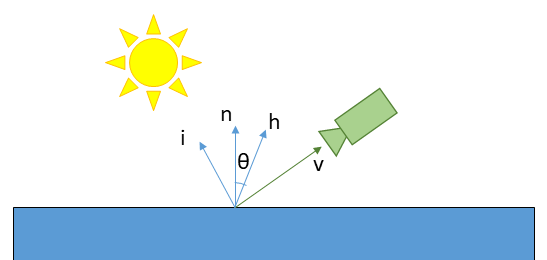
\includegraphics[width=\textwidth]{specular_angle}
		\end{column}
		\begin{column}{0.65\textwidth}
			\begin{itemize}
				\pause\item Let $h$ be the ``halfway vector'', calculated by $i+v$
				\pause\item The closer $h$ is to $n$, the higher the specular contribution.
			\end{itemize}
		\end{column}
	\end{columns}
	\begin{itemize}
		\pause\item Specular light intensity is proportional to
		$$ \operatorname{clamp}(n \cdot h)^s $$
		where $s$ is a ``shininess'' parameter, and $\operatorname{clamp}(x)$ clamps its argument between $0$ and $1$
	\end{itemize}
\end{frame}

\begin{frame}{Ambient lighting}
	\begin{itemize}
		\pause\item Currently, surfaces pointing away from the light are completely \textbf{black} (light intensity = 0)
		\pause\item In the real world, light scattered from one surface illuminates others
		\pause\item In the Phong model, we cheat and add a little \textbf{ambient} intensity to the lighting, which is just the light colour applied to the object colour with a constent ``ambient factor''.
		\pause\item Another option would be to add more light sources...
	\end{itemize}
\end{frame}

\begin{frame}{Normal mapping}
	\pause
	\begin{columns}
		\begin{column}{0.33\textwidth}
			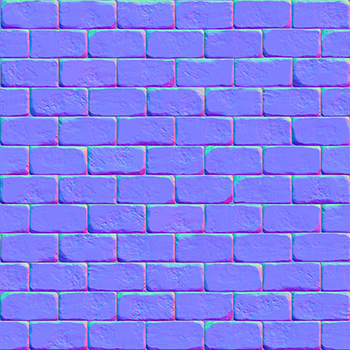
\includegraphics[width=\textwidth]{normal_map}
		\end{column}
		\begin{column}{0.65\textwidth}
			\begin{itemize}
				\item A \textbf{normal map} is a texture which is used to slightly alter the normal
					across a surface
					\begin{itemize}
						\pause\item Each pixel in the normal map represents a 3D vector, with $xyz$ mapped to RGB
					\end{itemize}
			\end{itemize}
		\end{column}
	\end{columns}
	\pause
	\begin{columns}
		\begin{column}{0.33\textwidth}
			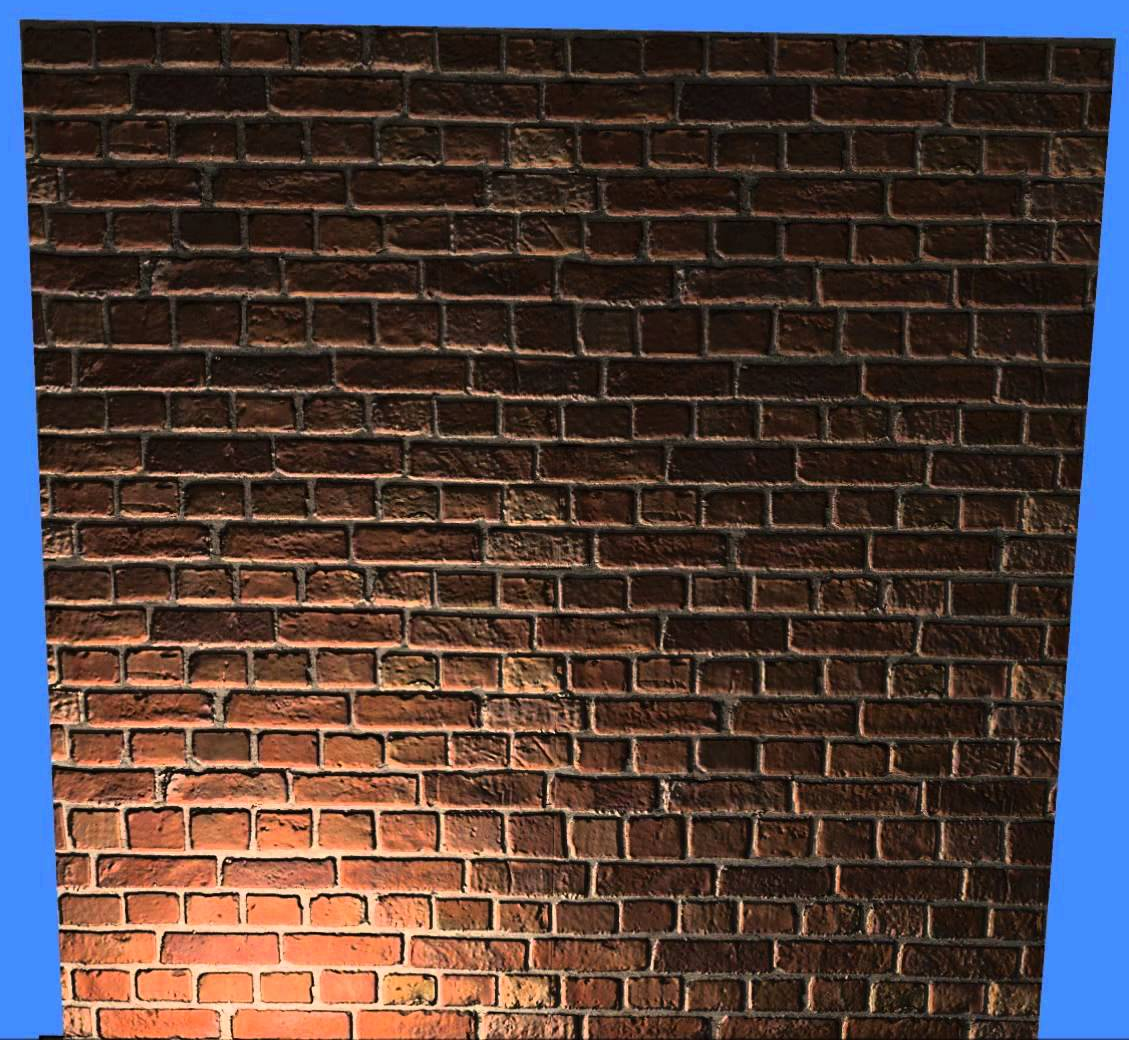
\includegraphics[width=\textwidth]{normal_mapped_wall}
		\end{column}
		\begin{column}{0.65\textwidth}
			\begin{itemize}
				\item Can be used to add detail to flat, low-poly surfaces
				\pause\item Can use textures to change other lighting parameters across a surface,
					e.g.\ \textbf{specular mapping}
			\end{itemize}
		\end{column}
	\end{columns}
\end{frame}
